\chapter{Cadenas de Markov ocultas y modelado computacional}
\label{chap:hmm}

En el capítulo anterior se introdujo el uso de cadenas de Markov como un primer modelo para la caracterización matemática de melodías musicales, considerando únicamente información observable. Bajo ese enfoque, la melodía se representó como una sucesión discreta de notas y se modeló la dependencia local entre notas consecutivas mediante probabilidades de transición. Esta aproximación es útil para capturar regularidades inmediatas (por ejemplo, preferencias por movimientos conjuntos o patrones repetitivos), pero presenta limitaciones cuando se busca incorporar estructuras musicales que organizan la melodía sin estar explícitamente codificadas en la secuencia de notas.

En particular, la armonía suele actuar como una estructura subyacente que condiciona la evolución melódica: aun cuando una melodía sea completamente observable, el \emph{contexto armónico} que la hace musicalmente coherente (acordes implícitos, función tonal, tensión y resolución) no aparece necesariamente como un símbolo explícito en cada instante. Desde un punto de vista probabilístico, esto sugiere que la secuencia observable está influida por un mecanismo interno no observable directamente.

Con el objetivo de extender el marco teórico y superar estas limitaciones, en este capítulo se introduce el modelo de cadenas de Markov ocultas. Este modelo permite formalizar la coexistencia de dos niveles de descripción: un proceso estocástico oculto que captura la estructura subyacente (interpretada aquí como \emph{estado armónico} o \emph{contexto musical latente}) y un proceso observable que se genera a partir de dicho estado oculto (interpretado aquí como \emph{nota} o símbolo melódico). Además, se introducen los problemas algorítmicos fundamentales que permiten realizar inferencia eficiente, lo cual constituye el puente hacia el desarrollo computacional del proyecto.

\begin{Definicion}
Sea $(\Omega,\mathcal{F},\mathbb{P})$ un espacio de probabilidad. Una cadena de Markov oculta está definida por dos procesos estocásticos en tiempo discreto
\[
(X_n)_{n \geq 0}, \qquad (Y_n)_{n \geq 0},
\]
donde $(X_n)$ es un proceso no observable directamente u ocultos, denominado proceso oculto, y $(Y_n)$ es un proceso observable. Se fija un espacio de estados ocultos finito
\[
\mathcal{S} = \{1,2,\dots,N\},
\]
y un espacio de observaciones discreto
\[
\mathcal{V} = \{v_1,v_2,\dots,v_M\}.
\]

El proceso $(X_n)$ satisface la propiedad de Markov, es decir, para todo $n \geq 0$ y para cualesquiera $i_0,\dots,i_{n+1} \in \mathcal{S}$,
\[
P(X_{n+1} = i_{n+1} \mid X_n = i_n, \dots, X_0 = i_0)
=
P(X_{n+1} = i_{n+1} \mid X_n = i_n).
\]
Por otro lado, el proceso observable $(Y_n)$ está condicionado únicamente por el estado oculto actual. En particular, se asume que, dado $X_n$, la variable aleatoria $Y_n$ es independiente del resto del historial del proceso.
Dicho de manera más explícita: una vez conocido el estado oculto actual $X_n$, información adicional sobre estados y observaciones pasadas no modifica la distribución de $Y_n$. En símbolos, el pasado influye en $Y_n$ sólo a través del estado latente presente.
\end{Definicion}

La interpretación musical que guiará este capítulo es la siguiente. El proceso oculto $(X_n)$ representa un \emph{estado musical subyacente} que organiza la melodía; por ejemplo, puede asociarse a una función armónica, a un acorde implícito o a una región tonal que evoluciona a lo largo del tiempo. El proceso observable $(Y_n)$ representa la \emph{secuencia de notas} efectivamente registrada en la partitura (o, más generalmente, símbolos musicales observables). En este sentido, la cadena de Markov oculta formaliza la idea de que las notas son observaciones generadas a partir de un contexto armónico latente, y que dicho contexto evoluciona con dependencia local.

Una cadena de Markov oculta queda completamente determinada por el conjunto de parámetros
\[
\lambda = (\boldsymbol{\pi}, \mathbf{A}, \mathbf{B}),
\]
donde:

\begin{itemize}
    \item $\boldsymbol{\pi} = (\pi_i)_{i \in \mathcal{S}}$ es la distribución inicial del proceso oculto, con
    \[
    \pi_i = P(X_0 = i), \qquad \sum_{i=1}^N \pi_i = 1.
    \]
    \item $\mathbf{A} = (a_{ij})_{i,j \in \mathcal{S}}$ es la matriz de transición del proceso oculto, donde
    \[
    a_{ij} = P(X_{n+1} = j \mid X_n = i), \qquad \sum_{j=1}^N a_{ij} = 1.
    \]
    \item $\mathbf{B} = (b_j(v))_{j \in \mathcal{S},\, v \in \mathcal{V}}$ es la matriz de emisión, definida por
    \[
    b_j(v) = P(Y_n = v \mid X_n = j), \qquad \sum_{v \in \mathcal{V}} b_j(v) = 1.
    \]
\end{itemize}

Desde la perspectiva musical, $\boldsymbol{\pi}$ describe cuál es el contexto armónico inicial más probable; $\mathbf{A}$ describe la dinámica de cambio de contexto (por ejemplo, qué funciones armónicas tienden a seguir a cuáles); y $\mathbf{B}$ describe cómo cada contexto latente \emph{favorece} ciertas notas observables, codificando una relación estadística entre armonía y melodía.

Bajo estas hipótesis, la distribución conjunta de una trayectoria oculta $x_{0:T}$ y una secuencia observada $y_{0:T}$ factoriza como
\[
P(X_{0:T} = x_{0:T}, Y_{0:T} = y_{0:T})
=
\pi_{x_0} b_{x_0}(y_0)
\prod_{t=1}^{T} a_{x_{t-1}x_t} b_{x_t}(y_t).
\]
(añadir referencias = bloc de notas)

Esta factorización explicita la lógica generativa del modelo: primero se selecciona un estado latente inicial $X_0$ según $\boldsymbol{\pi}$; luego el estado latente evoluciona según $\mathbf{A}$; y en cada instante se genera una observación $Y_t$ según la distribución de emisión determinada por el estado oculto actual. En música, esto equivale a postular que existe un ``hilo armónico'' que evoluciona localmente y que, en cada paso, produce notas con probabilidades características del contexto en curso.

Si se considera únicamente el proceso observable $(Y_n)_{n \geq 0}$, éste no satisface en general la propiedad de Markov. Esta afirmación es relevante musicalmente: aunque el contexto armónico evolucione con memoria corta, la secuencia de notas observable puede exhibir dependencias más complejas, precisamente porque ``hereda'' la memoria del estado latente.

\begin{proposition}
El proceso observable $(Y_n)_{n\ge 0}$ de una cadena de Markov oculta no es, en general, una cadena de Markov.
\end{proposition}

\begin{proof}
Basta dar un ejemplo donde falle la propiedad de Markov. Sea $\mathcal S=\{1,2\}$ y $\mathcal V=\{0,1\}$. Defínase el proceso oculto $(X_n)$ con
\[
A=\begin{pmatrix}1&0\\0&1\end{pmatrix},
\qquad
P(X_0=1)=P(X_0=2)=\tfrac12,
\]
de modo que $X_n=X_0$ para todo $n$.

Defínase el mecanismo de emisión por
\[
P(Y_n=1\mid X_n=1)=p,\qquad P(Y_n=1\mid X_n=2)=q,
\]
con $p\neq q$ y $p,q\in(0,1)$. Entonces, condicionado en $X_0=i$, las variables $(Y_n)$ son i.i.d.\ Bernoulli con parámetro $p$ si $i=1$ y con parámetro $q$ si $i=2$.

Calculemos ahora dos probabilidades condicionales. Por la ley de la probabilidad total,
\[
P(Y_2=1,\,Y_1=1,\,Y_0=1)
=
\tfrac12\,p^3+\tfrac12\,q^3,
\qquad
P(Y_1=1,\,Y_0=1)=\tfrac12\,p^2+\tfrac12\,q^2.
\]
Por lo tanto,
\[
P(Y_2=1\mid Y_1=1,\,Y_0=1)=\frac{p^3+q^3}{p^2+q^2}.
\]
De manera similar,
\[
P(Y_2=1,\,Y_1=1)=\tfrac12\,p^2+\tfrac12\,q^2,
\qquad
P(Y_1=1)=\tfrac12\,p+\tfrac12\,q,
\]
y así
\[
P(Y_2=1\mid Y_1=1)=\frac{p^2+q^2}{p+q}.
\]

Si $(Y_n)$ fuera Markov de primer orden, debería cumplirse
\[
P(Y_2=1\mid Y_1=1,\,Y_0=1)=P(Y_2=1\mid Y_1=1).
\]
Sin embargo, para $p,q\in(0,1)$ con $p\neq q$ se tiene la desigualdad estricta
\[
\frac{p^3+q^3}{p^2+q^2}>\frac{p^2+q^2}{p+q},
\]
pues, al desarrollar la expresión,
\[
(p^3+q^3)(p+q)-(p^2+q^2)^2
=
pq\,(p-q)^2>0.
\]
Concluimos que $P(Y_2=1\mid Y_1=1,\,Y_0=1)\neq P(Y_2=1\mid Y_1=1)$, y por tanto $(Y_n)$ no satisface la propiedad de Markov de primer orden.
\end{proof}

Esta pérdida de la propiedad de Markov no constituye una deficiencia del modelo, sino una consecuencia natural de la presencia de variables latentes. En el lenguaje musical, el contexto armónico oculto actúa como una ``memoria'' adicional: incluso si sólo se observa la nota actual, la probabilidad de la siguiente nota puede depender de información previa porque el estado armónico aún no está determinado unívocamente por una sola observación.

No obstante, si se considera el proceso conjunto $(Z_n)_{n \geq 0}$ definido por
\[
Z_n = (X_n, Y_n),
\]
entonces dicho proceso sí satisface la propiedad de Markov en el espacio producto $\mathcal{S} \times \mathcal{V}$. Este resultado se establece formalmente a continuación.

\begin{proposition}
El proceso $(Z_n)_{n \geq 0} = (X_n, Y_n)$ es una cadena de Markov en el espacio de estados $\mathcal{S} \times \mathcal{V}$.
\end{proposition}

\begin{proof}
Sean $(i,v),(j,w) \in \mathcal{S} \times \mathcal{V}$ y $n \geq 0$. Por definición,
\[
\begin{aligned}
P(Z_{n+1} = (j,w) &\mid Z_n = (i,v), Z_{n-1}, \dots, Z_0) \\
&= P(X_{n+1} = j, Y_{n+1} = w \mid X_n = i, Y_n = v, \dots).
\end{aligned}
\]
Utilizando la regla del producto y las hipótesis del modelo, se obtiene
\[
\begin{aligned}
P(X_{n+1} = j, Y_{n+1} = w &\mid X_n = i, Y_n = v, \dots) \\
&= P(Y_{n+1} = w \mid X_{n+1} = j)\, P(X_{n+1} = j \mid X_n = i).
\end{aligned}
\]
La igualdad anterior se justifica por dos hechos: primero, el proceso oculto $(X_n)$ satisface la propiedad de Markov, por lo que
\[
P(X_{n+1} = j \mid X_n = i, X_{n-1}, \dots) = a_{ij};
\]
segundo, las observaciones son condicionalmente independientes del pasado dado el estado oculto actual, lo que implica
\[
P(Y_{n+1} = w \mid X_{n+1} = j, X_n, Y_n, \dots) = b_j(w).
\]
Por lo tanto,
\[
\begin{aligned}
P(Z_{n+1} = (j,w) &\mid Z_n = (i,v), Z_{n-1}, \dots, Z_0) \\
&= a_{ij}\, b_j(w),
\end{aligned}
\]
lo cual depende únicamente del estado actual $Z_n = (i,v)$. Esto prueba que $(Z_n)$ satisface la propiedad de Markov. 
\end{proof}

Este resultado pone de manifiesto que una cadena de Markov oculta puede interpretarse como una cadena de Markov ordinaria en un espacio de estados ampliado, cuya estructura particular refleja la descomposición entre la dinámica oculta y la dinámica observable. En términos musicales, al considerar simultáneamente ``contexto armónico'' y ``nota observada'' se recupera una dinámica con memoria corta, aun cuando la observación por sí sola presente dependencias más largas. \cite{cappe2005}.

En el caso particular en el que la observación determina de manera única el estado oculto, es decir, cuando existe una función determinista $f : \mathcal{V} \to \mathcal{S}$ tal que $X_n = f(Y_n)$ casi seguramente para todo $n$, el proceso observable $(Y_n)$ hereda la propiedad de Markov. Esta situación corresponde, en música, a un escenario idealizado donde cada nota identifica sin ambigüedad el contexto armónico, lo cual raramente ocurre en repertorios reales pero es útil como caso límite.

\begin{proposition}
Supóngase que existe una función determinista $f:\mathcal V\to\mathcal S$ tal que
\[
X_n = f(Y_n) \quad \text{casi seguramente para todo } n\ge 0.
\]
Entonces, el proceso observable $(Y_n)_{n\ge 0}$ es una cadena de Markov de primer orden.
\end{proposition}

\begin{proof}
Sea $v_0,\dots,v_n,v_{n+1}\in\mathcal V$. Por hipótesis, el estado oculto queda determinado de manera única por la observación, es decir,
\[
X_k = f(Y_k)\quad \text{c.s. para todo } k.
\]
En particular, conocer $Y_n=v_n$ equivale a conocer $X_n=f(v_n)$.

Consideremos la probabilidad condicional
\[
P(Y_{n+1}=v_{n+1}\mid Y_n=v_n,Y_{n-1}=v_{n-1},\dots,Y_0=v_0).
\]
Usando la ley de la probabilidad total e introduciendo el estado oculto,
\[
P(Y_{n+1}=v_{n+1}\mid Y_n=v_n,\dots)
=
P(Y_{n+1}=v_{n+1}\mid X_n=f(v_n)).
\]
Esta igualdad se debe a que, dado $Y_n=v_n$, los valores pasados $Y_{n-1},\dots,Y_0$ no aportan información adicional sobre $X_n$, pues $X_n$ queda completamente determinado por $Y_n$.

Ahora bien, por la estructura del modelo de cadena de Markov oculta,
\[
\begin{aligned}
P(Y_{n+1}=v_{n+1}\mid X_n=f(v_n))
&=
\sum_{j\in\mathcal S}
P(Y_{n+1}=v_{n+1}\mid X_{n+1}=j)\, \\
&\qquad\qquad P(X_{n+1}=j\mid X_n=f(v_n)).
\end{aligned}
\]
El lado derecho depende únicamente de $v_n$, y no del historial previo de las observaciones. Por lo tanto,
\[
\begin{aligned}
P(Y_{n+1}=v_{n+1} &\mid Y_n=v_n,Y_{n-1},\dots,Y_0) \\
&= P(Y_{n+1}=v_{n+1}\mid Y_n=v_n),
\end{aligned}
\]
lo que prueba que $(Y_n)$ satisface la propiedad de Markov de primer orden.
\end{proof}

\begin{observacion}
La igualdad $X_n = f(Y_n)$ debe entenderse en el sentido de igualdad entre variables aleatorias, es decir, casi seguramente. Dado que $X_n$ y $Y_n$ son funciones definidas sobre un espacio de probabilidad común, exigir igualdad punto a punto no es necesario ni natural en este contexto. En efecto, dos variables aleatorias que difieren únicamente en un conjunto de probabilidad nula inducen las mismas probabilidades condicionales y, por tanto, son indistinguibles desde el punto de vista del análisis estocástico. En consecuencia, la hipótesis $X_n = f(Y_n)$ c.s.\ es suficiente para garantizar que la observación determina completamente el estado oculto a nivel probabilístico. \cite{cappe2005}
\end{observacion}

\section{Problemas fundamentales de Markov oculto}

Una vez fijado el modelo, las preguntas relevantes no son únicamente ``qué es'' una cadena de Markov oculta, sino qué se puede \emph{inferir} a partir de ella. En el contexto musical, esto se traduce en dos tareas centrales: cuantificar qué tan compatible es una secuencia de notas con un modelo (por ejemplo, con un estilo armónico-melódico aprendido) y reconstruir el contexto latente más probable que pudo haber generado la melodía observada. Ambas tareas se formalizan en los problemas clásicos de evaluación y decodificación.

Dado un modelo $\lambda$ y una secuencia observada $y_{0:T}$, se consideran tres problemas clásicos en la teoría de cadenas de Markov ocultas: evaluación, aprendizaje y decodificación. Para el presente trabajo los dos problemas más relevante son el de evaluación y decodificación. Aprendizaje fue un paradigma durante muchos años para modelos de inteligencia artificial pero estos han sido sobrepasados por tecnologías mas modernas, a continuación se explica en detalle estos problemas.

\subsection{Evaluación}

Sea un modelo
\[
\lambda = (\boldsymbol{\pi}, \mathbf{A}, \mathbf{B})
\]
y una secuencia de observaciones
\[
y_{1:T} = (y_1, y_2, \dots, y_T).
\]
El problema de evaluación consiste en determinar la probabilidad
\[
P(y_{1:T} \mid \lambda).
\]
En música, esta cantidad puede interpretarse como un puntaje de verosimilitud: mide qué tan plausible es la secuencia de notas observada bajo el modelo armónico-latente propuesto.

Aunque esta probabilidad puede calcularse directamente mediante argumentos probabilísticos clásicos, dicho enfoque requiere considerar todas las posibles trayectorias de estados ocultos, lo cual involucra $N^T$ operaciones y resulta computacionalmente inviable incluso para valores moderados de $T$. Este obstáculo es especialmente relevante en análisis musical, donde una melodía real puede tener cientos o miles de instantes discretos.

Para resolver este problema de manera eficiente se introduce una variable auxiliar $\alpha_t(i)$, denominada \emph{variable hacia adelante} (\emph{forward variable}), definida como
\[
\alpha_t(i) = P(y_1, y_2, \dots, y_t, X_t = i \mid \lambda).
\]
Estas variables satisfacen la siguiente relación recursiva:
\[
\alpha_{t+1}(j) = b_j(y_{t+1}) \sum_{i=1}^N \alpha_t(i)\, a_{ij},
\qquad 1 \le j \le N,\; 1 \le t \le T-1,
\]
con condiciones iniciales
\[
\alpha_1(j) = \pi_j\, b_j(y_1), \qquad 1 \le j \le N.
\]
La probabilidad total de la secuencia observada queda entonces dada por
\[
P(y_{1:T} \mid \lambda) = \sum_{i=1}^N \alpha_T(i).
\]
La complejidad computacional de este algoritmo es del orden $O(N^2T)$, lo cual representa una mejora exponencial con respecto al cálculo directo.

Desde el punto de vista interpretativo, $\alpha_t(i)$ cuantifica la probabilidad de que, tras escuchar (u observar) los primeros $t$ símbolos de la melodía, el estado armónico latente en el instante $t$ sea $i$. Así, el algoritmo \emph{forward} puede verse como un mecanismo de propagación de creencias sobre el contexto armónico conforme avanza la melodía.

\subsection{Decodificación }

El problema de decodificación en una cadena de Markov oculta consiste en determinar, dada una secuencia observada, una trayectoria de estados ocultos que maximice la probabilidad posterior. En el caso estándar, este problema se formula como la búsqueda de la trayectoria que maximiza la probabilidad conjunta con la secuencia observada.

En música, esta tarea se interpreta como la reconstrucción de la secuencia de contextos latentes más probable (por ejemplo, la progresión armónica implícita) que pudo haber generado las notas observadas, bajo el modelo $\lambda$. El algoritmo de Viterbi resuelve este problema de manera eficiente mediante programación dinámica. En lugar de enumerar todas las posibles trayectorias ocultas, cuya cantidad crece exponencialmente con la longitud de la secuencia, el algoritmo explota la estructura markoviana del modelo para construir soluciones óptimas parciales que se combinan recursivamente.

Sea $y_{0:T}$ una secuencia observada. Se define
\[
\delta_t(j) = \max_{x_{0:t-1}} P(X_{0:t-1} = x_{0:t-1}, X_t = j, Y_{0:t} = y_{0:t}),
\]
con condiciones iniciales
\[
\delta_0(j) = \pi_j b_j(y_0),
\]
y la recurrencia
\[
\delta_t(j) = b_j(y_t) \max_{i \in \mathcal{S}} \delta_{t-1}(i) a_{ij}.
\]
La trayectoria óptima se obtiene mediante un procedimiento de retroceso a partir de
\[
\hat{x}_T = \arg\max_{j \in \mathcal{S}} \delta_T(j).
\]
Las ecuaciones anteriores describen la lógica del método; el pseudocódigo siguiente resume su implementación paso a paso.

\begin{algorithm}[H]
\caption{Algoritmo de Viterbi}
\label{alg:viterbi}
\begin{algorithmic}[1]
\Require Observaciones $O=(o_1,\dots,o_T)$, estados $S=\{1,\dots,N\}$,
probabilidades iniciales $\boldsymbol{\pi}$, matriz de transición $A=(a_{ij})$,
probabilidades de emisión $B=(b_j)$
\Ensure Secuencia de estados más probable $X^*=(x_1^*,\dots,x_T^*)$

\Statex
\State \textbf{Inicialización}
\For{$j = 1$ \textbf{to} $N$}
    \State $\delta_1(j) \gets \pi_j\, b_j(o_1)$
    \State $\psi_1(j) \gets 0$
\EndFor

\Statex
\State \textbf{Recursión}
\For{$t = 2$ \textbf{to} $T$}
    \For{$j = 1$ \textbf{to} $N$}
        \State $\displaystyle 
        \delta_t(j) \gets 
        \max_{1 \le i \le N} \bigl[ \delta_{t-1}(i)\, a_{ij} \bigr]\; b_j(o_t)$
        \State $\displaystyle 
        \psi_t(j) \gets 
        \arg\max_{1 \le i \le N} \bigl[ \delta_{t-1}(i)\, a_{ij} \bigr]$
    \EndFor
\EndFor

\Statex
\State \textbf{Terminación}
\State $\displaystyle P^* \gets \max_{1 \le j \le N} \delta_T(j)$
\State $\displaystyle x_T^* \gets \arg\max_{1 \le j \le N} \delta_T(j)$

\Statex
\State \textbf{Retropropagación}
\For{$t = T-1, T-2, \dots, 1$}
    \State $x_t^* \gets \psi_{t+1}(x_{t+1}^*)$
\EndFor

\Statex
\Return $X^* = (x_1^*,\dots,x_T^*)$
\end{algorithmic}
\end{algorithm}
\cite{bouguila2020}

En términos musicales, el resultado de Viterbi entrega la ``explicación latente'' más probable de la melodía: una trayectoria $X^*$ que puede interpretarse como la secuencia de contextos armónicos que mejor justifica las notas observadas bajo el modelo. Esto es particularmente valioso cuando se desea comparar interpretaciones armónicas implícitas o estudiar cómo cambia la estructura subyacente a lo largo de una pieza.

El modelo oculto encuentra una limitación importante: puede ocurrir que algunos estados latentes no sean efectivamente visitados o inferidos a partir de los datos disponibles. Dado que los estados ocultos suelen representar clases de contexto (por ejemplo, funciones o configuraciones armónicas), es posible que ciertas configuraciones nunca aparezcan en una pieza o en un corpus pequeño, lo cual induce probabilidades de transición o emisión nulas en una estimación puramente frecuentista. Este fenómeno no sólo es computacional (porque puede bloquear trayectorias en Viterbi), sino también interpretativo (porque restringe artificialmente el espacio de explicaciones armónicas). A continuación se presenta un ejemplo de este caso.

Se realizó una prueba con la pieza \emph{Preludio en Do Mayor} de J.\,S. Bach (1685--1750) utilizando los siguientes parámetros. La matriz de transición $\mathbf{A}=(A_{ij})$ se define sobre los \emph{estados ocultos} (interpretados aquí como acordes, o triadas de notas). En este tipo de estudios es común imponer una estructura homogénea de la forma
\begin{equation}
A_{ii} \;=\; \frac{\alpha}{\alpha+(N-1)\beta},
\qquad
A_{ij} \;=\; \frac{\beta}{\alpha+(N-1)\beta}\quad (i\neq j),
\label{eq:transicion_alpha_beta}
\end{equation}
donde $N=\lvert\mathcal{S}\rvert$ es el número de estados ocultos. Aquí $\alpha$ controla la permanencia en el mismo estado, mientras que $\beta$ regula la probabilidad de transición hacia estados distintos. Con esta parametrización, la probabilidad de \emph{cambiar} de acorde en un paso es baja, mientras que la probabilidad de \emph{permanecer} en el mismo acorde es alta.

En nuestro caso fijamos $\alpha=210$ y $\beta=1$, y tomamos una distribución inicial uniforme,
\[
\pi_i=\frac{1}{N},\qquad i=1,\dots,N.
\]
Esta elección significa que, al inicio, ningún acorde se privilegia \emph{a priori} sobre otro: antes de observar la secuencia, todos los estados ocultos se consideran igualmente plausibles.
Por ejemplo, si $N=24$, entonces
\[
A_{ii}=\frac{210}{210+23}\approx 0.901,
\qquad
\sum_{j\neq i}A_{ij}=\frac{23}{210+23}\approx 0.099,
\]
es decir, la probabilidad de quedarse en el mismo acorde es aproximadamente $0.9$ y la de moverse a un acorde distinto es aproximadamente $0.1$.

Se analizó esta pieza debido a que el conteo manual de las transiciones armónicas resulta relativamente accesible. Esto permite construir una matriz de transición “real” basada directamente en la partitura y utilizarla como referencia para evaluar el desempeño del modelo oculto. De esta manera, se dispone de un criterio empírico claro para comparar la estructura armónica inferida algorítmicamente con la estructura efectivamente observada en la obra.

El procedimiento seguido fue el siguiente. Primero, se identificó manualmente la sucesión de acordes presentes en la pieza y se construyó la matriz de transiciones empírica mediante conteo directo y normalización por renglones. Posteriormente, utilizando el modelo de cadena de Markov oculta con los parámetros previamente especificados, se aplicó el algoritmo de Viterbi para obtener la trayectoria latente más probable de estados armónicos. A partir de esta trayectoria inferida, se reconstruyó la matriz de transiciones correspondiente y se comparó con la matriz real.

\bigskip

\begin{figure}[H]
    \centering
    \begin{subfigure}{0.9\textwidth}
        \centering
        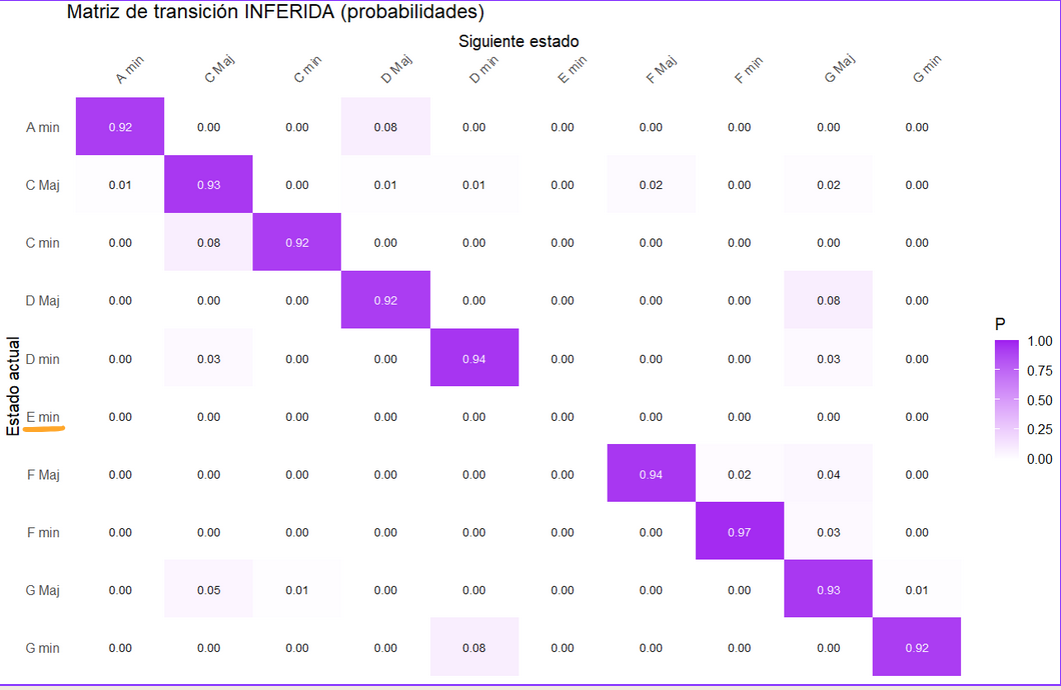
\includegraphics[width=\linewidth]{figures/Inferida.png}
        \caption{Matriz inferida mediante Viterbi}
        \label{fig:matriz_inferida}
    \end{subfigure}
    
    \medskip
    \begin{subfigure}{0.9\textwidth}
        \centering
        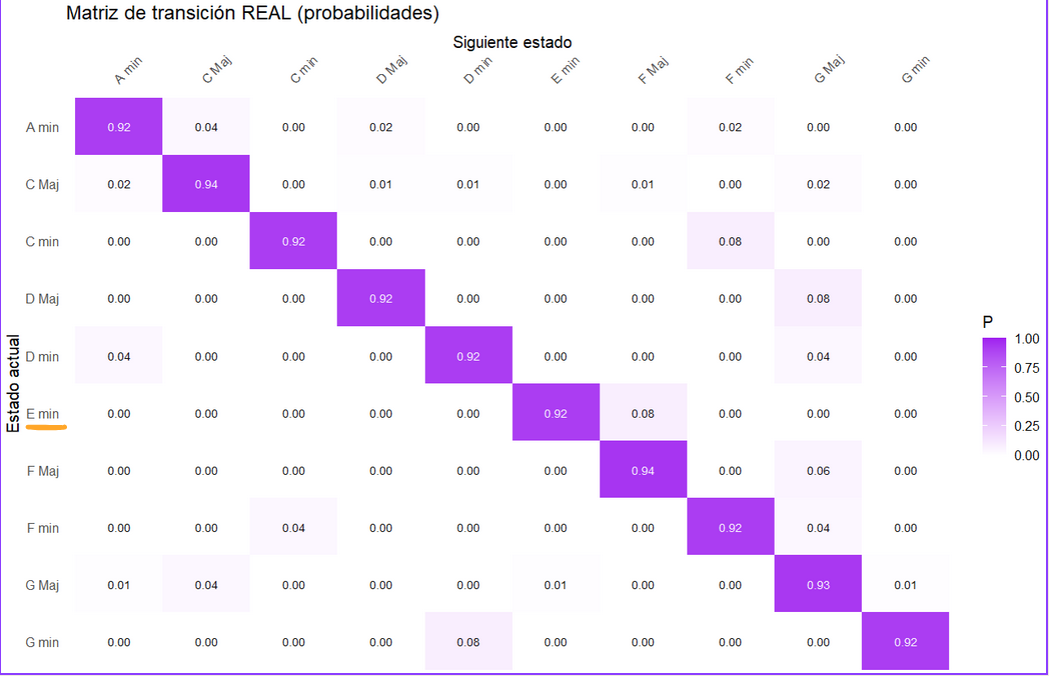
\includegraphics[width=\linewidth]{figures/real.png}
        \caption{Matriz real de transiciones}
        \label{fig:matriz_real}
    \end{subfigure}
    \caption{Comparación entre la matriz de transiciones armónicas inferida por el modelo oculto y la matriz obtenida mediante conteo directo de la partitura. En ambas, los tonos más oscuros indican probabilidades de transición más altas.}
    \label{fig:comparacion_matrices}
\end{figure}

\newpage

La comparación entre ambas matrices muestra con claridad tanto el alcance como la limitación del método. El modelo no observa acordes de manera directa, sino únicamente notas emitidas por estados latentes; por ello, la reconstrucción armónica que obtiene es necesariamente parcial. Aun así, las probabilidades dominantes, en particular las entradas diagonales asociadas a permanencia y varias de las transiciones estructuralmente frecuentes, coinciden cualitativamente con la matriz obtenida por conteo directo. Esto sugiere que la hipótesis de una dinámica markoviana latente resulta razonable para esta pieza. En total, la obra presenta $30$ cambios de acorde; el algoritmo identifica $27$ de ellos, es decir, el $90\%$. Entre esas $27$ transiciones detectadas, $22$ coinciden con la referencia manual, lo que equivale aproximadamente al $82\%$.

\bigskip    


\FloatBarrier
\begin{figure}[H]
    \centering
    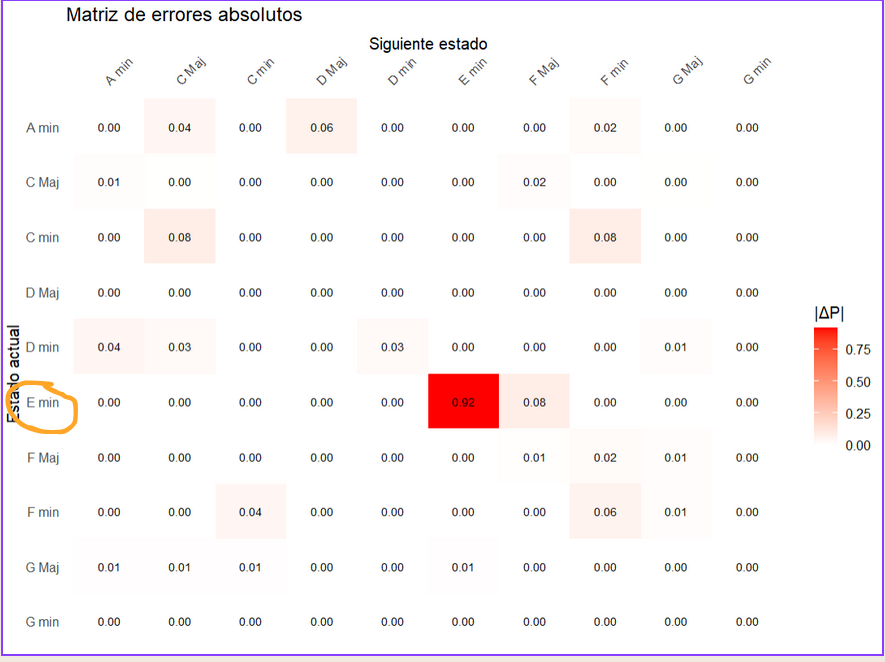
\includegraphics[width=0.82\linewidth]{figures/Error.png}
    \caption{Matriz de error de la estimación.}
    \label{fig:MatrizErr}
\end{figure}
\FloatBarrier

Esta limitación fundamental pone en evidencia la necesidad de expandir el alcance del modelo tradicional. Con el propósito de superar estas deficiencias estructurales, se ha propuesto diversas extensiones orientadas a dotar de mayor capacidad expresiva a las cadenas de Markov ocultas. 

En particular, una de estas alternativas consiste en las cadenas de Markov ocultas infinitas. Este modelo relaja la restricción de operar sobre un espacio de estados finito, asumiendo, en su lugar, una cardinalidad infinita para el conjunto de estados latentes. La premisa subyacente es que dicha formulación proporciona una representación armónica de mayor fidelidad, en tanto permite estimar y modelar la diversidad inherente de configuraciones musicales (como los acordes) con mayor precisión.

Conviene subrayar que el paso hacia este nuevo modelo no abandona la lógica desarrollada en el presente capítulo. Hasta aquí, la pregunta central ha sido: dado un HMM ya especificado, ¿cómo evaluar una secuencia observada y cómo reconstruir su trayectoria latente más probable? El capítulo siguiente conserva exactamente esa intuición musical, pero desplaza la dificultad a un nivel anterior: antes de inferir, hay que decidir cuántos estados armónicos necesita realmente el modelo para describir una pieza o un corpus sin colapsar distinciones relevantes ni inflar artificialmente el vocabulario.

Dicho de otro modo, el problema ya no será solamente \emph{cómo inferir} estados ocultos, sino también \emph{cuánta complejidad latente conviene permitir}. Esa pregunta conduce de manera natural al marco no paramétrico bayesiano: en lugar de fijar de antemano un inventario cerrado de contextos armónicos, se busca que la complejidad efectiva del modelo emerja de los datos observados.
